
To illustrate LIDL capabilities, we will use it to describe a simple graphical user interface (GUI). The example is a typical speed controller. Three modes are available: 

\begin{itemize}
\item \mono{Off}: Manual control of the speed
\item \mono{Lim}: Limiter, the speed should stay under a certain value
\item \mono{Ctrl}: Controller, the speed should stay around a certain value
\end{itemize}

Three buttons are available to control the target speed:
\begin{itemize}
\item \mono{+} to increment the target speed
\item \mono{-} to decrement the target speed
\item \mono{Cur} to set the target speed to the current actual speed
\end{itemize}


\begin{figure}
\begin{center}
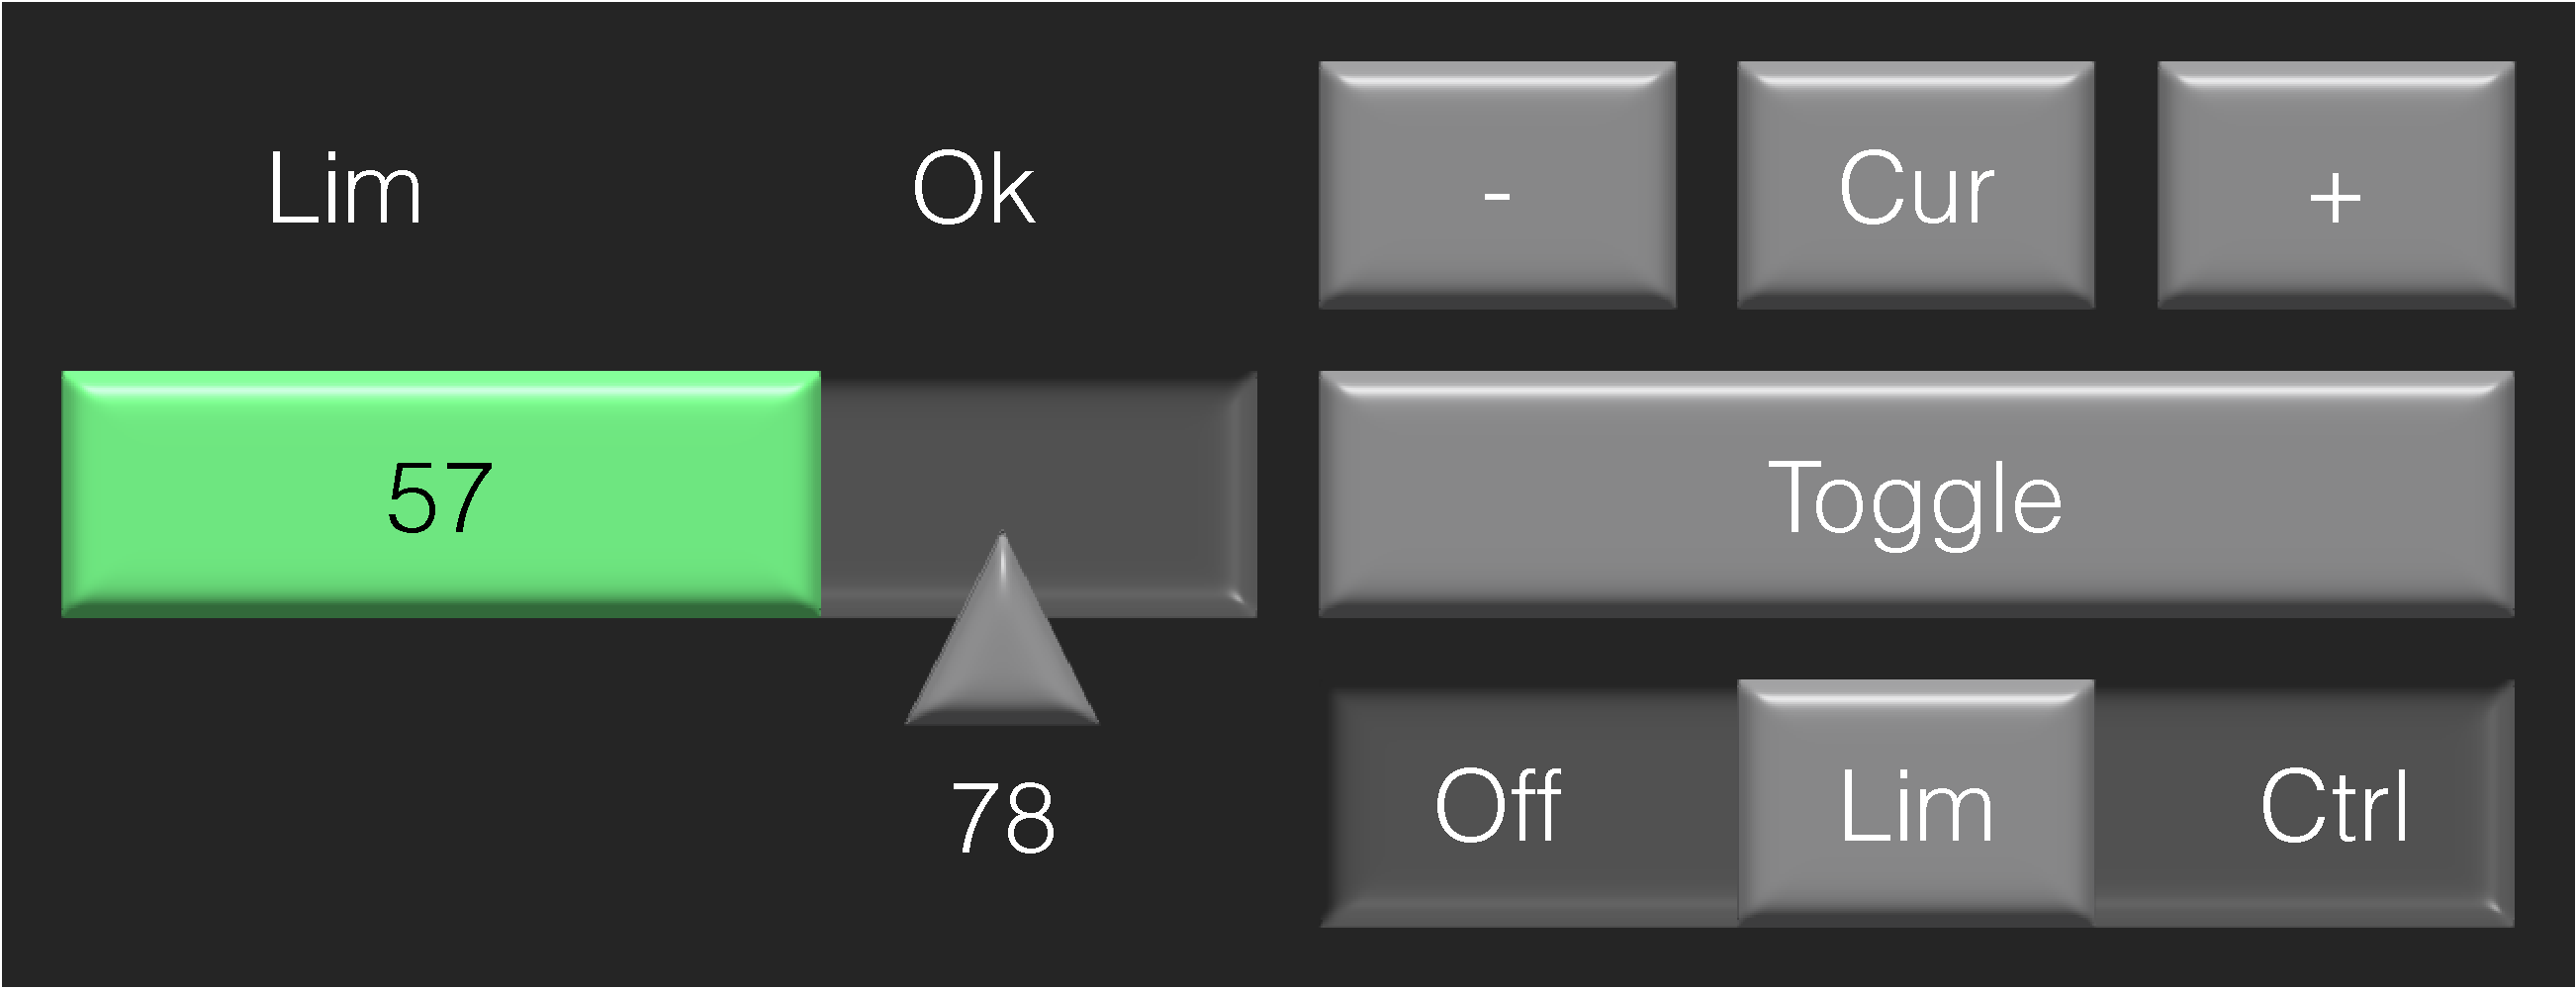
\includegraphics[width=\columnwidth,page=1]{drawings.pdf}
\end{center}
\caption{A mockup of the example GUI}
\label{fig-gui-example}
\end{figure}

\clearpage

\begin{lstlisting}[caption=Interface of the speed controller]
interface 
	SpeedController
is
	{
		system: {
			desiredMode:	text out,
			desiredSpeed:	number out,
			actualMode:		text in,
			actualSpeed:	number in
		},
		user: {
			mode:	Label,
			status:	Label,
			actual:	Gauge,
			desired:	Slider,
			increment:	Button,
			decrement:	Button,
			current:	Button,
			toggle:	Button,
			switch:	SegmentedSwitch
		}
	}
\end{lstlisting}

\clearpage

\begin{lstlisting}[caption=The speed controller interaction]
interaction 
	(TheSpeedController)
implementing
	SpeedController
is
	(bind ({
		system:{
			desiredMode: (theDesiredMode),
			desiredSpeed: (theDesiredSpeed),
			actualMode: (theActualMode),
			actualSpeed: (theActualSpeed)          
		},
		user:{	
			mode: (Label (active) 
				with value (theActualMode)),	
			status: (Label (active) 
				with value (
					if ((theActualMode) != (theDesiredMode))
					then ("Wrong mode")
					else if (((theDesiredMode) != ("Off")) 
					and((theActualSpeed)>(theDesiredSpeed)))
					then ("Over speed")
					else ("Ok")
				)),
			actual: (Gauge (active) 
				with value (theActualSpeed)),
			desired: (Slider (active) 
				with value (theDesiredSpeed)
				selecting (new(theDesiredSpeed))),
			increment: (Button (active) 
				with text ("+")
				triggering ( (new(theDesiredSpeed)) = 
				((previous(theDesiredSpeed))+(5)))),
			decrement: (Button (active) 
				with text ("-")
				triggering ( (new(theDesiredSpeed)) = 
				((previous(theDesiredSpeed))-(5)))),
			current: (Button (active) 
				with text ("Cur")
				triggering ( (new(theDesiredSpeed)) = 
				(round (theActualSpeed) to (5)))),
			toggle: (Button (active) 
				with text ("Toggle")
				triggering ( (new(theDesiredMode))=(
					if((previous(theDesiredMode))==("Off"))
					then(theSelectedMode)
					else("Off")
				))),
			switch: (SegmentedSwitch (active) 
				with choices (["Off","Lim","Ctrl"]) 
				selecting (theSelectedMode))
		}
	}) : (all
		(make (theDesiredSpeed) flow)  
		(make (theDesiredMode) flow) 
	))
\end{lstlisting}


\clearpage

\begin{lstlisting}[caption=The speed controller interaction unfolded]
interaction 
	(TheSpeedController)
implementing
	SpeedController
is
	(bind ({
		system:{
			desiredMode: (theDesiredMode),
			desiredSpeed: (theDesiredSpeed),
			actualMode: (theActualMode),
			actualSpeed: (theActualSpeed)          
		},
		user:{	
			mode: 	
				(bind(x1) : 
					((all
						((x1.value)=(theActualMode))
					)=(active))),
			status: 
				(bind(x2) : 
					((all((x2.value)=(if ((theActualMode) != (theDesiredMode))
						then ("Wrong mode")
						else if (((theDesiredMode) != ("Off")) and((theActualSpeed)>(theDesiredSpeed)))
						then ("Over speed")
						else ("Ok")))
					)=(active))),
			actual: 
				(bind(x3) : 
					((all
						((x3.value)=(theActualSpeed))
					)=(active))),
			desired:
				(bind(x4) : (
					(all
						((x4.value)=(theDesiredSpeed))
						((new(theDesiredSpeed))=(x4.selection))
					)=(active))),
			increment: 
				(bind(x5) : (
					(all((x5.value)=("+"))(((new(theDesiredSpeed))=((previous(theDesiredSpeed))+(5)))=(x5.click)))=(active))),
			decrement: 
				(bind(x6) : (
					(all((x6.value)=("-"))(((new(theDesiredSpeed))=((previous(theDesiredSpeed))-(5)))=(x6.click)))=(active))),
			current: 
				(bind(x7) : (
					(all((x7.value)=("Cur"))(((new(theDesiredSpeed))=(round (theActualSpeed) to (5)))=(x7.click)))=(active))),
			toggle: 
				(bind(x8) : (
					(all((x8.value)=("Toggle"))(
					( (new(theDesiredMode))=(
						if((previous(theDesiredMode))==("Off"))
						then(theSelectedMode)
						else("Off")
					))=(x8.click)))=(active))),
			switch: 
				(bind(x9) : ((all
					((x9.choices)=(["Off","Lim","Ctrl"]))
					((theSelectedMode)=((["Off","Lim","Ctrl"])[(x9.selection)])))=(active))),		
		}
	}) : (all
		((theDesiredSpeed) = 
			(if ((new(theDesiredSpeed)) is active) 
			then (new(theDesiredSpeed)) 
			else (previous(theDesiredSpeed))))
		((theDesiredMode) = 
			(if ((new(theDesiredMode)) is active) 
			then (new(theDesiredMode)) 
			else (previous(theDesiredMode))))
	))
\end{lstlisting}

Once totally unfolded, the SpeedController uses the following base interactions :

\begin{itemize}
	\item \code{bind\$:\$}
	\item \code{\$=\$}
	\item \code{all\$\$}
	\item \code{if\$then\$else\$}
	\item \code{previous\$}
	\item \code{\$+\$}
	\item \code{\$-\$}
	\item \code{\$==\$}
	\item \code{\$and\$}
	\item \code{round\$to\$}
	\item \code{\{system:\{desiredMode:\$,desiredSpeed:\$...\},user:\{...\}\}}
	\item \code{5}
	\item \code{active}
	\item \code{"Wrong Mode"}
	\item Other constants...
\end{itemize}


\clearpage
